\chapter{The ALICE experiment at the LHC}

\section{The Large Hadron Collider}
\iffalse
The Large Hadron Collider (LHC), with a circumference of 27 km, 
is the world's largest and most powerful particle collider, built by the 
European Organisation for Nuclear Research (CERN) from 1998 to 2008. \\It is placed in the tunnel of the previous Large Electron Positron collider, at a depth between 50 and 175 m underground.

The LHC accelerator chain is shown in fig. \ref{fig:imageLHC}. The first stage of the acceleration takes place on the Linac2, a linear accelerator with an output proton energy of 50 MeV. The proton-booster synchrotron (PSB) increases the energy to 1.4 GeV, injecting into the proton synchrotron (PS). This accelerates the beam to 26 GeV and injects into the super proton synchrotron (SPS), out of which 450 GeV protons are eventually injected into the LHC for the start of the ramp up to the energy of 7 TeV. Protons are grouped in 2808 bunches per beam, each bunch containing up to $10^{11}$ protons. The beam is bent along the circular LHC path by 1232 superconducting dipoles and controlled and focused by another 600 smaller magnets. The design and construction of the dipoles was the most technologically challenging part of the accelerator. To achieve the required bending power, the dipoles’ field should be on average B$\sim$8.3 Tesla. The coils are made of NiTi superconducting cable, kept at T=1.9K bysuperfluid liquid He. They are 15 m long, weigh 35 tonnes and store in their magnetic field 7 MJ of energy, for a total of ∌10 GJ in the full ring.\\
The nominal luminosity for p-p collisions is of $10^{34} s^{-1} cm^{-2}$ , while for Pb-Pb collisions it is about $10^{27} s^{-1} cm^{-2}$. \\Since September 2008, p-p beams circulated in the LHC ring at $\sqrt{s}=900, 2.36, 2.76, 7$ and 8 TeV, Pb-Pb beams at $\sqrt{s_{NN}}=2.76$ TeV and p-Pb beams at $\sqrt{s_{NN}}=5.02$ TeV.
\\
The main experiments running at the LHC are:
\begin{itemize}
\item \textbf{a Toroidal LArge Solenoid (ATLAS)}, its main goal is the search and the study of the Higgs boson and supersymmetric particles; 
\item \textbf{a Compact Muon Solenoid (CMS)}, dedicated to the study of the Higgs boson, supersymmetric and other beyond Standard Model particles;
\item \textbf{A Large Heavy Ion Collider Experiment (ALICE)}, entirely dedicated to the study of heavy ion physics;
\item \textbf{LHC-beauty (LHCb)}, designed to study CP violation in the sector of b-hadrons.
\end{itemize}
\begin{figure}[!t]
\centering
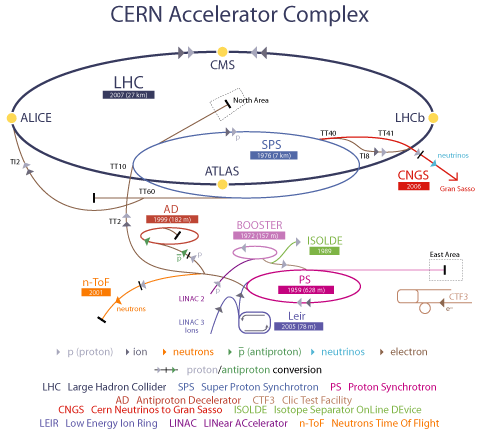
\includegraphics[width=12cm]{CERN_Accl_Complex.png}
\caption{Layout of the full CERN accelerator complex, including all elements of the LHC injector chain.}
\label{fig:imageLHC}
\end{figure} 
\section{The ALICE experiment}
ALICE (A Large Ion Collider Experiment) \cite{ALICEperf-May2014} is an experiment at the Large Hadron Collider optimized for the study of heavy-ion collisions, at a centre-of-mass energy $\sim$5.5 TeV per nucleon.
The aim of ALICE to study the behaviour of matter at high densities and temperatures and at near zero baryochemical potential led to the design of a detector consisting of three main components: 
\begin{itemize}
\item \textbf{The central barrel}, contained in the large magnet with a weak solenoidal field (0.5 T) and composed of detectors devoted to the study of hadronic signals and dielectrons and covering the pseudorapidity range -0.9$< \eta <$0.9 over the full azimuth. These are the \textit{Inner Tracking System} (ITS), optimized for vertex reconstruction and tracking; a cylindrical \textit{Time Projection Chamber} (TPC), surrounding the ITS, that is the most important detector for tracking; a \textit{Transition Radiation Detector} (TRD), designed for electron identification; a \textit{Time Of Flight} (TOF) detector, that provides pion, proton and kaon identification; a \textit{Photon Spectrometer} (PHOS); an \textit{Electromagnetic Calorimeter} (EMCal), a \textit{High-Momentum Particle IDentification} (HMPID) and the \textit{ALICE Cosmic Ray Detector} (ACORDE).
\item \textbf{The forward muon spectrometer}, mainly dedicated to the study of the muon pairs from the decay of quarkonia, covering the pseudorapidity range 2.5$< \eta <$4.0.
\item \textbf{The forward detectors}, which include the \textit{Photon Multiplicity Detector} (PMD) and the silicon \textit{Forward Multiplicity Detector} (FMD), dedicated to the measurement of photons and charged particles around $|\eta| \sim 3$, respectively; the quartz Cherenkov detector \textit{T0} delivers the time and the longitudinal position of the interaction; the plastic scintillator detector \textit{V0} measures charged particles at -3.7$< \eta <$-1.7 and 2.8$< \eta <$5.1, and is mainly used for triggering and for the determination of centrality and event plane angle in Pb-Pb collisions; the \textit{Zero Degree Calorimeter} (ZDC) also used for determination of centrality.
\end{itemize}
The layout of ALICE set-up is shown in fig. \ref{fig:imageALICE}. 
\begin{figure}[!t]
\centering
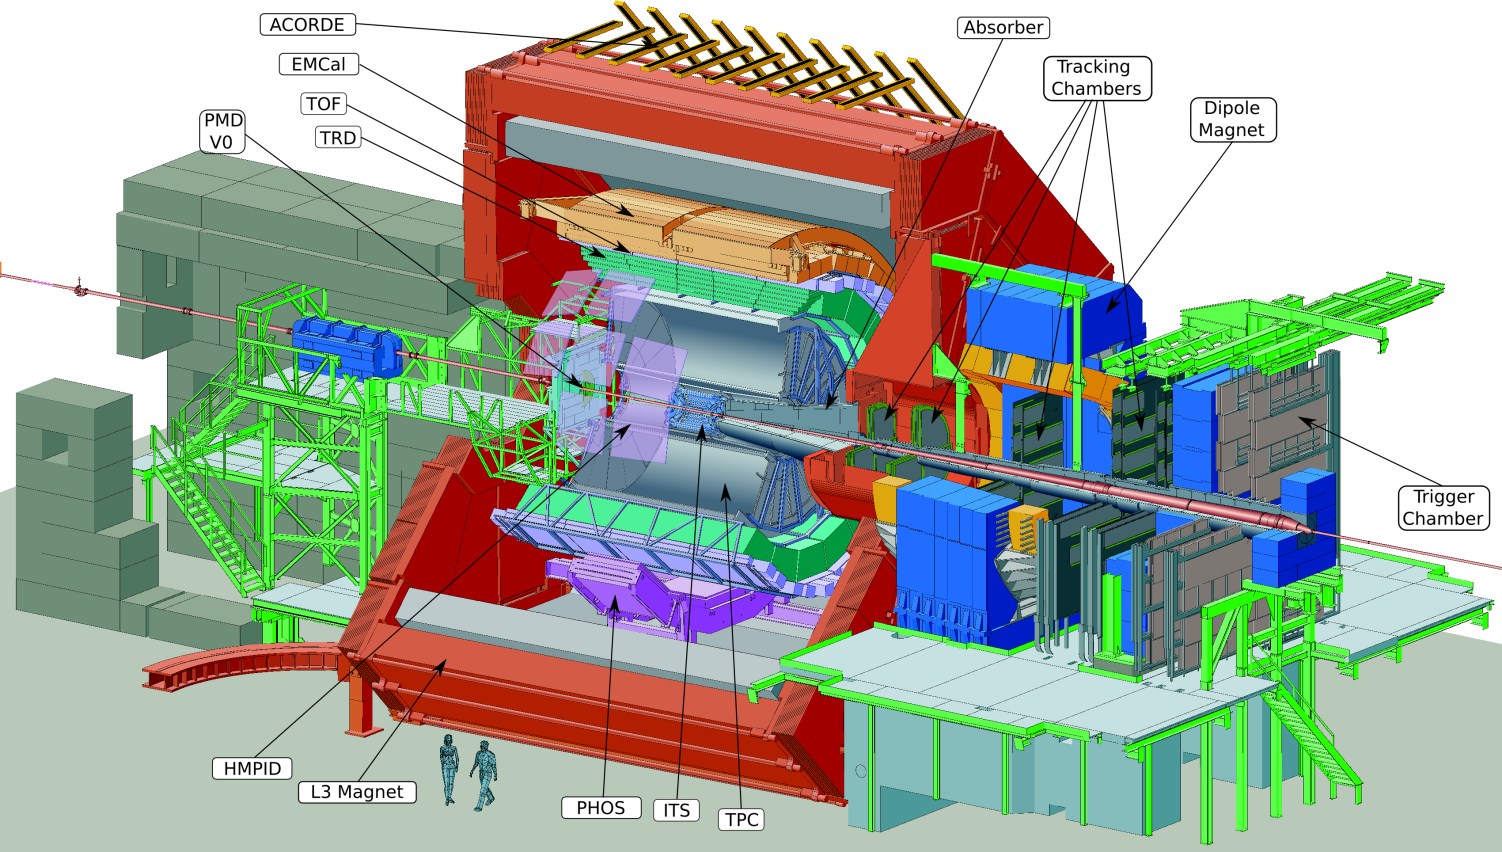
\includegraphics[width=12cm]{alice.png}
\caption{Picture of the ALICE experiment detectors.}
\label{fig:imageALICE}
\end{figure}
ALICE apparatus has overall dimensions of 16 x 16 x 26 $m^3$ and a total weight of $\sim$10000 t. The maximum p-p interaction rate at which all ALICE detectors can be safely operated is around 700 kHz. Typical luminosity values for the ALICE p-p data taking range from \textit{L}$\sim 10^{29}s^{-1}cm^{-2}$ to \textit{L}$\sim 10^{31}s^{-1}cm^{-2}$.
The rate of Pb-Pb collisions in 2010 and 2011 was well below the ALICE limits and ALICE was able to take data at the highest achievable luminosity, on the order of $10^{25}s^{-1}cm^{-2}$ in 2010 and $\sim 10^{26}s^{-1}cm^{-2}$ in 2011  \cite{ALICEperf-May2014}.
The major challenge the detector project had faced was the large number of particles created in Pb-Pb collisions. The design of the experiment was based on the highest value of particle production, 8000 charged particles per unit of rapidity, at midrapidity. For this reason, ALICE detectors was design to have a high granularity, a low transverse momentum threshold $p^{min}_t \sim 0.15 $ GeV/c and good particle identification capabilities up to 20 GeV/c.

In the following sections, the detectors of ALICE and their performance are described more in details.

\subsection{Magnet}
The magnet used in ALICE was constructed for the L3 experiment at LEP and it produces a relatively weak solenoidal magnetic field (B $<$ 0.5 T). In the choice of the magnetic field two aspects must be considered: the magnet has to be intense enough to bend the particle trajectory, but still to permit the reconstruction of low momentum particles. The lower momentum that allows reconstruction of the track with the ALICE magnet is given by $p_{cutoff}=0.3$ B$\cdot$R$\sim 0.2$ GeV/c, where B is the magnetic field in Tesla, R is the minimum radius for a particle to traverse the entire TPC, whose external radius is $R_{ext}=$ 2.5 m.


\subsection{Inner Tracking System (ITS)}
The Inner Tracking System of ALICE is one of the central detectors used for track reconstruction, primary and secondary vertex finding and Particle Identification (PID).
It surrounds the beam pipe, its basic functions are \cite{ITS-TDR}:
\begin{itemize}
\item determination of primary and secondary vertexes for charm, beauty and hyperon decay reconstruction,
\item particle identification and tracking of low-momentum particles,
\item improvement of the momentum and angle measurements of the TPC.
\end{itemize}
Because of high values of charged particle production occurring in Pb-Pb collisions, track finding is one the most challenging tasks in ALICE, and it is done by both the ITS and the Time Projection Chamber (TPC). Particle identification is done by different detectors in different momentum ranges. The ITS contributes to PID in the lower momentum range (up to 500 MeV/c). An example distribution of measured truncated mean energy loss values as a function of momentum in the ITS is shown in fig. \ref{fig:imagePIDITSTPC}. Finally, secondary vertex finding is a unique task of the ITS. \\
\begin{figure}[!t]
\centering
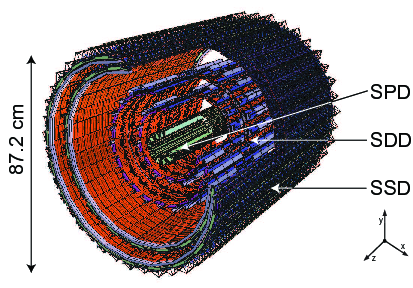
\includegraphics[width=8cm]{figures_its-rf-2.png}
\caption{View of the six silicon layers of the Inner Tracking System}
\label{fig:image2}
\end{figure}



The ITS is composed by six cylindrical layers of silicon detectors placed coaxially around the beam pipe (fig. \ref{fig:image2}). The layers are located at radii between 39 mm and 430 mm and cover the pseudorapidity range $|\eta|<0.9$. The two innermost layers are made of Silicon Pixel Detectors (SPD), their pseudorapidity coverage is $|\eta|<1.95$.% An
%example distribution of measured truncated mean energy loss values as a function of momentum in the ITS is shown in fig. \ref{fig:imagePIDITSTPC}.
The two middle layers are made of Silicon Drift Detectors (SDD) and two outer layers of Silicon micro-Strip Detectors (SSD).
\begin{figure}[b]
\begin{subfigure}{0.5\textwidth}
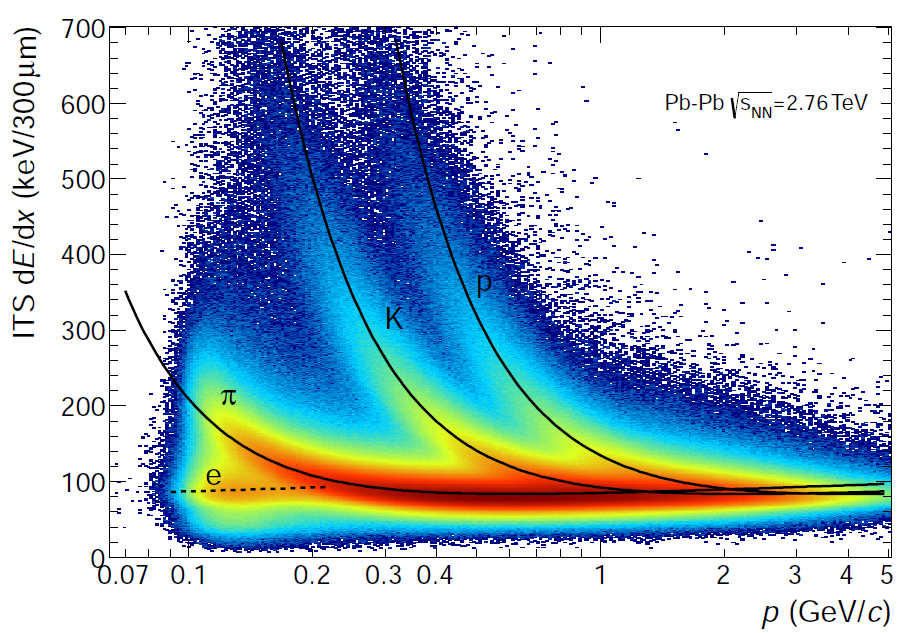
\includegraphics[width=7cm]{ITSpid.png}
\end{subfigure}
\begin{subfigure}{0.5\textwidth}
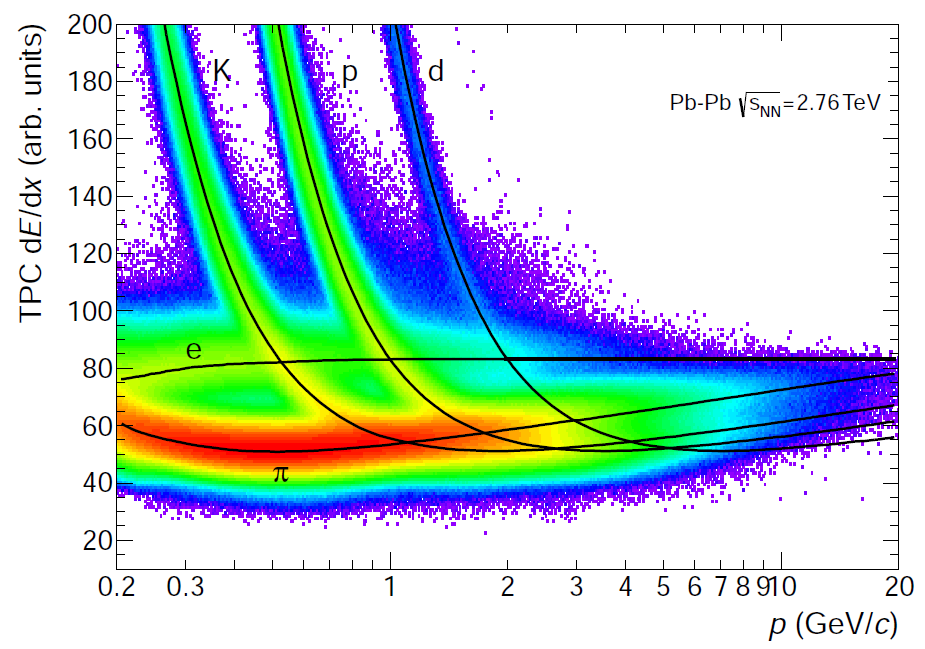
\includegraphics[width=7cm]{TPCpid.png}
\end{subfigure}
\caption{Distribution of the energy-loss signal in the ITS (left) and TPC (right) as a function of momentum. The lines show the parametrizations of the expected mean energy loss.}
\label{fig:imagePIDITSTPC}
\end{figure}


 The four outer layers have analogue read-out and for this reason they can be used for particle identification (PID) via dE/dx measurements for low-$p_t$ particles. The measured cluster charge is normalized to the path length, which is calculated from the reconstructed track parameters to obtain a dE/dx value for each layer. All detectors were carefully optimised to minimise their radiation length, achieving 1.1\% per layer, the lowest value among all the current LHC experiments \cite{ITS-TDRUp}. 
\\



The resolution of the impact parameter is determined by the spatial resolution of the ITS detectors. The ITS detectors have a spatial resolution of a few tens of $\mu$m in the $r\phi$ plane, with the best precision (12  $\mu$m) for the innermost detectors. All ITS detectors have a resolution in the plane perpendicular to the beam axis one order of magnitude better than that of the TPC, which in turn provides many more points.


\subsection{Time Projection Chamber (TPC)}
The need for a large number of points on each track has led to the choice of a TPC as the main tracking system. It is the only device which can provide good performance up to 8000 charged particles per unit of rapidity  \cite{TPC-TDR}. 



It has a cylindrical shape with inner and outer radius of 80 and 250 cm, respectively, and an overall length in the beam direction of 500 cm. The minimum possible inner radius of the TPC is given by the maximum acceptable hit density. The outer radius is determined by the minimum length required for a dE/dx resolution better than 10\%. At smaller radii (and larger track densities), tracking is taken over by the ITS.\\It covers an acceptance of $|\eta|<0.9$. The TPC is a  chamber full of high-purity gas to transport primary charges over long distences (2.5 m) towards the read-out end-plates. 
The TPC it is composed by a central high-voltage (HV) electrode which divides the gas volume into two symmetric drift regions, and two opposite axial potential degraders create a highly uniform electrostatic field of up to 400 V/cm (fig. \ref{fig:image3} left).\\
Charged particles traversing the gas form a ionization trace that will move at constant velocity towards one of the two end-plates. The density of ionization depends on the velocity and mass of the particle.
Once on the "end-plate", readout chambers allow to amplify and register the signals of particle tracks.  The end-plates are equipped with wire planes and 560,000 electronics channels, detecting the fundamental properties of the ionization trace (3D image and ionization density). They are segmented into 18 trapezoidal sectors and equipped with multi-wire proportional chambers covering an overall active area of 32.5 $m^2$.
The mixture of gas is composed by 90\% Ne, 10\% $CO_2$; more recently a 5\% $N_2$ was added in order to improve drift velocity. This gas mixture needs a high drift field (400 V/cm) to secure an acceptable drift time (92$\mu$s for the last mixture). It is very important to provide high stability and uniformity in this mixture as they influence the precision in track reconstruction and energy-loss measurements. 


\begin{figure}[!t]
\begin{subfigure}{0.5\textwidth}
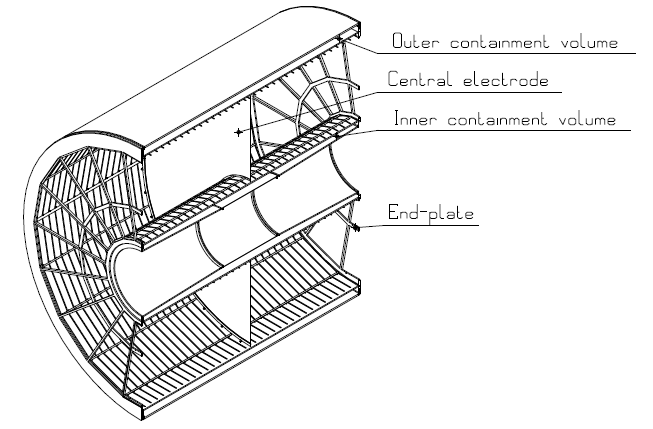
\includegraphics[width=8cm]{TPC.png}
\end{subfigure}
\begin{subfigure}{0.5\textwidth}
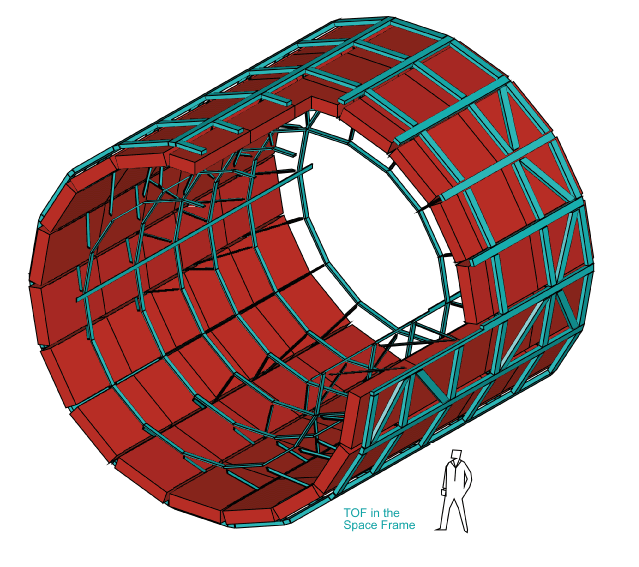
\includegraphics[width=6cm]{TOFCylinder.png}
\end{subfigure}
\caption{A view of the ALICE Time-Projection Chamber (left) and Time-Of-Flight (right) detector.}
\label{fig:image3}
\end{figure}
The TPC provides track finding (efficiency larger than 90\%), charged particle momentum measurement (resolution better than 2.5\% for electrons with momentum of about 4 GeV/c), particle identification (dE/dx resolution better than 10\%), and two-track separation (resolution in relative momentum below 5 MeV/c) in the region $p_t<10$ GeV/c.
Particle Identification is perfomed over a wide momentum range. It is made by measuring the specific energy loss, the charge and the momentum of each particle traversing the detector gas. Figure \ref{fig:imagePIDITSTPC} (right) shows the measured dE/dx vs particle momentum in the TPC, and it is evident the clear separation between the different particle species. The lines correspond to the parametrization. Thanks to the dE/dx resolution, particle ratios can be measured at a $p_t$ of up to 20 GeV/c.

\subsection{Transition Radiation Detector (TRD)}
The Transition Radiation Detector \cite{TRD-TDR} is placed between the Time Projection Chamber and the Time-Of-Flight detectors. It is the main detector in the central barrel revealing high momentum electrons, with $p_t >$1 GeV/c, i.e. the region where it is no more possible to use only the information from energy loss of TPC for particle identification. Since the TRD is a fast tracker, it is possible to use it as an efficient trigger for high-momentum electrons. As the other detectors of the barrel, the TRD covers an acceptance of $|\eta|<$0.9.
The transition radiation is produced when a highly relativistic charged particle traverses the boundary between two media of different dielectric constants. The probability of transition radiation increases with the relativistic gamma factor and this provides an excellent way to discriminate between electrons and pions for momenta of a few GeV/c and higher. The probability of emission traversing a single boundary is small, so multiple boundaries are necessary to obtain a reasonable efficiency.
It consists of 540 detector modules, each one composed by a radiator of 4.8 cm thickness, a multi-wire proportional readout chamber, and the front-end electronics for this chamber. The gas mixture in the readout chamber is Xe/CO\textsubscript{2} (85\%/15\%). Each readout chamber consists of a drift region of 3.0 cm separated by cathode wires from an amplification region of 0.7 cm. The drift time is 2.0 $\mu$s.
\begin{figure}[b]
\centering
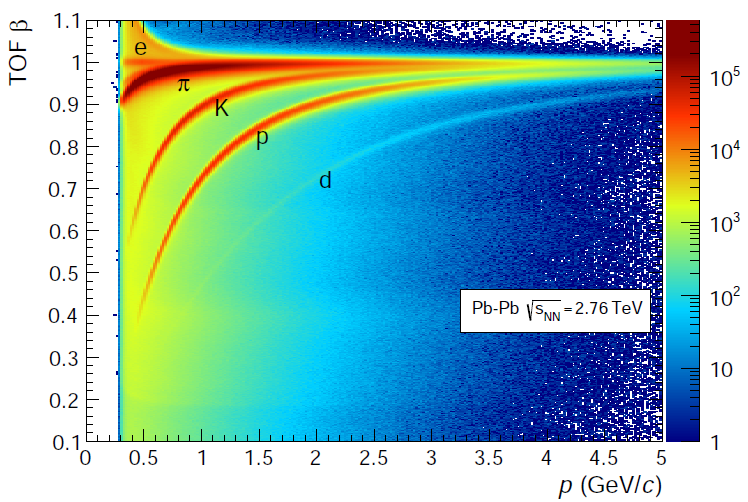
\includegraphics[width=8cm]{TOFpid.png}
\caption{Distribution of $\Beta$ as measured by the TOF detector as a function of momentum for particles reaching the
TOF in Pb–Pb interactions.}
\label{fig:TOFpid}
\end{figure}


\subsection{Time-Of-Flight (TOF)}
Among ALICE detectors, two of them are entirely devoted to the particle identification, a TOF array for momenta between 0.5 GeV/c (upper limit for dE/dx measurements in both the ITS and the TPC) and 2.5 GeV/c for pions and kaons, 4 GeV/c for protons and a small system (HMPID) for higher momenta. The TOF has a cylindrical shape, covering polar angles between 45 and 135 degrees over the full azimuth. It has a modular structure with 18 sectors in $\phi$ (fig. \ref{fig:image3} right); each of these sectors is divided into 5 modules along the beam direction. The modules contain a total of 1638 detector elements (MRPC strips), covering an area of 160 $m^2$ with 157248 readout channels (pads). The ionization produced by any particle crossing the MRPCs starts a gas avalanche which generates the observed signal. 
The TOF identifies the particle species via a measure of the time of flight 
inside the chambers. Considering the following relation:
\[
m = p \sqrt{\frac{t^2_{TOF}}{L^2}-1}
\]
where m is the mass of the particle, p the momentum, $t_{TOF}$ the time-of-flight and L  the track length, it is simple to show that the $\delta m/m$ resolution, at relatively high momenta, it is influenced much more by the errors on the time-of-flight and track length measurements than by error on the momentum determination.\\
The TOF intrisic time resolution is around 100 ps, and this implies a 3 sigma separation up to 1.9 GeV/c for kaon/pion and up to 3.2 GeV/c for proton/kaon.\\
Figure \ref{fig:TOFpid} illustrates the performance of the TOF detector. It is shown the measured velocity $\Beta$ distribution as a function of momentum (measured by TPC). The background is due to tracks that are incorrectly matched to TOF hits in high-multiplicity Pb-Pb collisions.

\subsection{High Momentum Particle Identification (HMPID)}
The High Momentum Particle Identification system plays a role in the particle identification of heavy-ion collisions in ALICE \cite{HMPID-TDR}. It allows to extend the PID capabilities beyond the momentum range allowed by energy loss measurements (ITS and TPC, $p \sim$ 600 MeV/c) and by the TOF ($p \sim$ 1.2-1.4 GeV/c). The HMPID detector has been designed to extend the useful range for identification of $\pi$/K up to 3 GeV/c and of p/K up to 5 GeV/c. 


This detector consists of seven modules of about 1.5$\times$1.5 m\textsuperscript{2} each of Ring Imaging Cherenkov (RICH) counters. Cherenkov radiation is a wave resulting from charged particles when traversing a material faster than the velocity of light in that material. The radiation propagates with a characteristics angle, that depends on the particle velocity. The radiator is a thick layer of $C_6F_{14}$ (perfluorohexane) with an index of refraction $n$=1.2989 at $\lambda$=175 nm, corresponding to a momentum threshold of $p_{th}$=1.21$\times$m, where m is the particle mass. Then, a photon detector made of CsI is used to detect the ring-shaped image of the Cherenkov radiation. From a measurement of the Cherenkov angle and thus the particle velocity, the mass of the charged particle can be estimated.

\subsection{Photon Spectrometer (PHOS)}
PHOS (PHOton Spectrometer) is an electromagnetic calorimeter of high granularity made of lead tungstate crystals \cite{PHOS-TDR}. It is positioned at the bottom of the ALICE set-up and covers about a quarter of unit in pseudorapidity, $-0.12<\eta<0.12$ and $100°$ in azimuthal angle. The main aim of the PHOS detector is the determination of the thermal and dynamical properties of the initial phase of the collision. This is done by measuring photons emerging directly from the collisions, that have to be separated by photons coming from particle decays, and also neutral mesons like $\pi^0$ and $\eta$ through their decays in two photons.

\subsection{Electromagnetic Calorimeter (EMCal)}
The Electromagnetic Calorimeter EMCal enhances ALICE's capabilities for jet quenching measurements \cite{EMCal-TDR}.
The detector contains several modules each consisting of sampling calorimeters, in fact the EMCal extends the ALICE $p_t$ capabilities for jets, direct photons and electrons from heavy-flavour decays. It is made of alternating layers of 1.44 mm Pb and 1.76 mm polystyrene, which is the scintillating material. The EMCal covers the pseudorapidity range $-0.7 < \eta < 0.7$.

\subsection{Forward Muon Spectrometer (FMS)}
The Forward Muon Spectrometer is used to evaluate the production of $\mu^+\mu^-$ pairs coming from the decay of heavy quarkonium states, like the charmonium states (J/$\Psi$ and $\Psi'$) and the bottomonium states ($\Upsilon, \Upsilon'$ and $ \Upsilon"$). In presence of a deconfined medium, quarkonium states are dissociated because of colour  screening and this leads to a suppression of their production rates.

The spectrometer is located around the beam pipe and its acceptance covers the pseudorapidity interval 2.5$\leq \eta \leq$4 \cite{FMS-TDR}. A resolution of 70 MeV/$c^2$ in the 3 GeV/$c^2$ region is needed to separate J/$\Psi$ and $\Psi'$ peaks and of 100 MeV/$c^2$ in the 10 GeV/$c^2$ region to distinguish $\Upsilon, \Upsilon' $and $\Upsilon"$.
This detector is composed by a front absorber (fig. \ref{fig:muon} left) which suppresses all the particles except the muons. It is made by carbon and concrete in order to limit the energy loss and multiple scattering of the muons. Then, a tracking chamber allows to obtain muon tracks, thanks to multi-wire proportional chambers, with a spatial resolution better than 100 $\mu$m, and a dipole magnet outside the L3 magnet which bends the charged particles tracks. The trigger on dimuon signals is provided by four layers of RPC operating in streamer mode that are located behind an iron absorber.
\begin{figure}[!t]
\begin{subfigure}{0.5\textwidth}
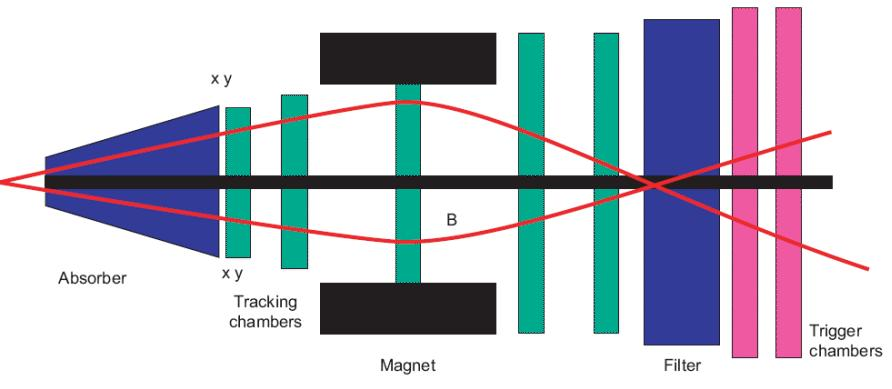
\includegraphics[width=8cm]{dimuon1.jpeg}
\end{subfigure}
\begin{subfigure}{0.5\textwidth}
\centering
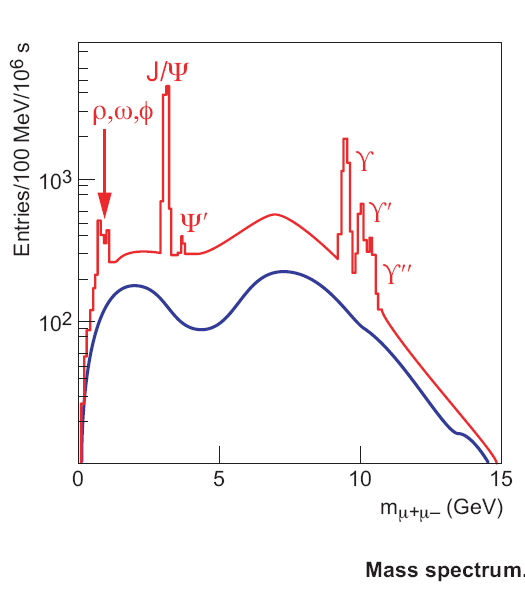
\includegraphics[width=5cm]{dimuon2.png}
\end{subfigure}
\caption{(Left) Basic principle of the Dimuon spectrometer: an absorber to filter the background, a set of tracking chambers before, inside and after the magnet and a set of trigger chambers. (Right) Mass spectrum of principal resonances of quarkonium states.}
\label{fig:muon}
\end{figure}


\subsection{Forward rapidity and trigger detectors}
To complete the ALICE apparatus there are still some detectors placed at small angles with respect to the beam  axis.
\\
\\
The \textbf{ZDCs Zero Degree Calorimeters} provide a measure of the number of spectator nucleons in the collision, useful to estimate the centrality of the event \cite{ZDC-TDR}. Typically the beams are deflected by means of two separation dipoles at a certain distance from the interaction point (IP). These magnets will also deflect the spectator protons, separating them from the spectator neutrons, which basically fly away at 0◩. Hence, two ZDCs are placed between the separation dipoles, 115 m away from the interaction point on both sides of the IP: one of them, positioned between the two beams to intercept the spectator neutrons, and the other one, external to the outgoing beam, to collect the spectator protons. \\The active material of the calorimeters is made of quartz fibres, while the passive one is made of metal plates.
\\
\\
The \textbf{V0 Detector} \cite{V0T0-TDR} is made of two arrays of scintillator counters set on both sides of the ALICE interaction point, and called V0L and V0R respectively. It provides a minimum bias trigger for the central barrel detectors and can be used to estimate the centrality of the collision by summing up the energy deposited in the two V0.
\\
\\
The \textbf{T0 detector} \cite{V0T0-TDR}, made of 24 Cherenkov radiators, generates the T0 signal for the TOF detector with a precision of ∌ 50 ps, measures a rough vertex position, provides a first level trigger and helps to discriminate against beam-gas interactions.
\\
\\
The \textbf{Photon Multiplicity Detector (PMD)} \cite{PMD-TDR}, designed to measure the multiplicity and the spatial distribution of photons, in the pseudorapidity region $ 2.3 < \eta < 3.7$. It consists of a charged particle veto (CPV) and a preshower plane to identify photons with full azimuth coverage. It is placed on the L3 magnet door 5.8 m from the interaction point on the opposite side of the dimuon spectrometer. The PMD cannot be used as a trigger because of its slow readout.
\\
\\
The \textbf{Forward Multiplicity Detector (FMD)} measures the charged-particle multiplicity over a large fraction of phase space, $-3.4 < \eta < -1.7$ and $1.7 < \eta < 5.0$, both in full azimuth \cite{V0T0-TDR}. The detector is composed of silicon strips located in five rings at z = 3.2 m, 0.83 m, 0.75 m, -0.63 m and -0.75 m. Due to its slow readout ($>$ 1.2 $\mu$s) it cannot be used as a trigger.

\section{The ALICE Trigger System and Data Aquisition}
ALICE has a two-layer trigger architecture \cite{trigger-TDR}. The low-level trigger is a hardware trigger called Central Trigger Processor (CTP). The High-Level trigger (HLT) is implemented as a pure software trigger. 
The ALICE Central Trigger Processor (CTP) is designed to combine and synchronize information from all the triggering detectors in ALICE, and to send the correct sequences of trigger signals to all detectors in order to make them read-out properly. As the ALICE experiment has to do with p-p and Pb-Pb collisions, the trigger system was optimized for both these types of collisions. The HLT allows the implementation of sophisticated logic for the triggering. While the CTP governs the readout of the subdetectors, the HLT receives a copy of the data read out from the subdetectors and processes it.

\subsection{The Central Trigger Processor (CTP)}
The hardware trigger combines informations from subdetectors to decide whether or not to write an event on disk. The trigger inputs are divided into three different levels, because of the dimension of the detector:
\begin{itemize}
\item L0 level: everything that can be decided within 1.2 $\mu$s after the collision has taken place is used to make the L0 decision. The trigger requirement can be simply the input of one detector or a logical condition based on the trigger inputs of different trigger detectors.
\item L1 level: for those detectors which require a longer time, 6.5 $\mu$s after the collision.
\item L2 level: a third step, which comes after about 88 $\mu$s, it is used to avoid a \textit{pile-up} effect, due to both the high luminosity and the slowness of some detectors. For example, in the TPC, which is the slowest detector with a drift time of 88 $\mu$s, charges from the previous event can be found together with charges of the interesting event. For not having to deal with these problems, the CTP invokes the "past-future protection" that rejects any other event when in a time window centered on the considered event. The sensitive periods for each detector have to be taken into account, since the past-future protection depends on them.
\end{itemize}
Several triggers (central, semi-central and minimum bias) are so frequent that the limiting factor is the performance of the data acquisition system. These triggers will use a very large fraction of the total data acquisition bandwidth. On the other hand, rare triggers such as dimuon or dielectron events, use less bandwidth and are limited by the detector livetime and the luminosity. By definition minimum-bias triggers have the highest rate of inputs signals, other triggers that look for rare signals have much lower rate. To prevent losing precious events due to the fact that no space is available on the temporary memory and disk buffers in a moment where a trigger that looks for a rare signal occurs, the trigger system implements an event prioritization scheme. Therefore, trigger classes are grouped into common triggers and rare triggers \cite{trigger2}. In the case that the utilization of the temporary storage is above a certain value, only rare triggers are accepted; as soon as the utilization drops below a given level all triggers are accepted again. This scheme significantly increases the acceptance of rare events.
Only when the L2 requirements are fulfilled, the event can be sent to the Data Aquisition System (DAQ). The DAQ manages the data flow from the subdetector electronics to the archiving on tape.

\subsection{The Data AcQuisition System (DAQ)}
The DAQ manages the data flow from the subdetector electronics to the archiving on tape. Once the CTP decides to register a specifice event, raw data are sent to the Local Data Concentrators (LDCs) via the optical Detector Data Links (DDLs). LDCs are sets of computers that perform sub-event reconstruction. In this step of the acquisition, raw data are processed. The event fragments processed by LDCs are then transferred to a second layer of computers, the Global Data Collectors (GDCs) which perform the event building. At this moment, the data rate coming from the different subdetectors is about 25 GB/s and the size of a single central event can be ≈ 70 MB. In order to optimize the use of the recording bandwidth available, an additional event selection and compression is done by the High-Level Trigger (HLT).

\subsection{The High Level Trigger (HLT)}
ALICE’s software trigger, called HLT, is a farm of multiprocessor computers. It is composed by about 1000 PCs processing the data in parallel allowing an online analysis of the events. A trigger decision is derived from much more complete information than is available for the hardware trigger. Therefore, it allows for more sophisticated triggers. Examples include triggers on high-energy jets or on muon pairs. Data rate reduction is achieved by reducing the event rate by selecting interesting events (software trigger) and by reducing the event size by selecting sub-events (e.g. pile-up removal in pp interactions) and by advanced data compression. 
\\
\\
The HLT receives a copy of the raw data and performs per detector reconstruction. Then, the trigger decision is based on the global reconstructed event. In the last optional step, if the trigger decision is positive, the data is compressed. The trigger decision, partial readout information, compressed data, and the reconstruction output is sent to LDCs and subsequently processed by the DAQ. 

\section{The ALICE Offline Software Framework}
The data production of the LHC experiments (about 10-15 PB per year) is at a new scale compared to any previous experiment. \\In ALICE, an average Pb-Pb event will have a size of about 13.75 MB; on average a p-p event is about 1.1 MB. For a standard running year, an order of $10^9$ p-p events and $10^8$ Pb-Pb events are expected, for a total raw data volume of 2.5 PB. The processing and analysis of these data necessitate unprecedented amount of computing and storage resources. Grid computing provides the answer to these needs. Grid computing consists of a coordinated use of large sets of different, geographically distributed resources in order to allow high-performance computation. It is organised in different levels or Tiers. Data coming from LHC experiments are stored in the CERN computing centre, the Tier-0. Copies of the collected data are then replicated in large regional computing centres (Tier-1), which also contribute in the event reconstruction and Monte Carlo simulation. Tier-2 centres are computing centres located in different institutions which do not have large storage capabilities but provide a large fraction of the computing resources for Monte Carlo simulation, data reconstruction and data analysis. \\ALICE uses the ALICE Environment (AliEn) system \cite{alien} as a user interface to connect to a Grid composed of ALICE specific services that are part of the AliEn framework and basic services of the Grid middleware installed at the different sites.

\subsection{The AliRoot Framework}
The ALICE offline framework, AliRoot \cite{trigger2} is based on Object-Oriented techniques for programming and, as a supporting framework, on the ROOT system \cite{root}, complemented by the AliEn system which gives access to the computing Grid. The AliRoot framework was developed as an extension of ROOT and is used for simulation, alignment, calibration, reconstruction, visualisation and analysis of the experimental data.
\begin{figure}[h]
\centering
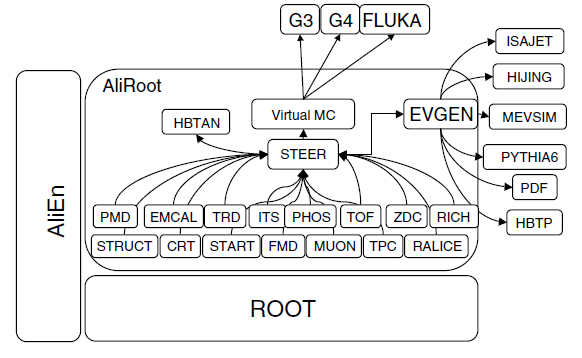
\includegraphics[width=10cm]{aliroot.png}
\caption{Schematic view of the AliRoot framework.}
\label{fig:aliroot}
\end{figure}
TheAliRoot framework is schematically shown in figure \ref{fig:aliroot}. The STEER module provides steering, run management, interface classes, and base classes. The detectors are independent modules that contain the code for simulation and reconstruction while the analysis code is progressively added. Detector response simulation can be performed via different transport  packages like GEANT3 \cite{geant3} and FLUKA \cite{fluka} written in FORTRAN and GEANT4 \cite{geant4} written in C++. In these packages the detector material budget is simulated in detail, including support structures and the beam pipe. The transport code can hence simulate the decays of unstable particles and the trajectory of the daughter particles, the interactions of the particles with the detectors material and the production of secondary electrons.\\
The reconstruction results are stored in ESDs (Event Summary Data), from which the analysis task produce the AODs (Analysis Object Data) specialised in the physics objectives and used for the analysis (for example, specific AOD are produced for the reconstruction of open-charm meson with two or three body decays).


\section{Event generators}
Event generators provide simulated events that are as close as possible to real interactions as occur at the collision point. Generated events are used to obtain an understanding of the data and signals that are expected, for preparing the analysis strategies and implementing the needed analysis code, as well as for estimating the needed corrections to obtain from the raw measurements the true signal. In addition, results of event generators together with further simulation software are used to plan and optimize the detector design. \\Since ALICE has to do with proton-proton, proton-nucleus and nucleus-nucleus collisions, simulation tools must include generators for all the interaction topologies.
As different theoretical models exist that give different predictions for the expected multiplicity in nucleus-nucleus collisions at LHC, different generators with different predictions for multiplicity, $p_t$ and rapidity distributions were developed.
The existing generators do not exactly simulate several fenomena also because the physics behind them is still not completely clear.\\
The main generators used for hadron-hadron collisions are PYTHIA \cite{pythia} and HERWIG \cite{herwig}. The available generators for heavy-ion interactions are: HIJING \cite{hijing}, DPMJET (Dual Parton Model Jet) \cite{DPMJET} and SFM (String Fusion Model) \cite{SFM}. \\ The generators used for the study presented here are HIJING and PYTHIA. \\ \\ {\bf PYTHIA} is used for simulation of particle production from proton-proton interactions. Since not all the physics processes are calculable because of non-perturbative contributions, the generator includes both analytical results and QCD-based models. Pythia contains theoretical perturbative QCD calculations that are exact only at leading order, where only the \textit{pair creation} processes, $q\=q \rightarrow Q\=Q$ and $gg \rightarrow Q\=Q$, are included. High-order contributions at the next-to-leading order are however included in this generator, allowing accounting for flavour excitation processes like $qQ \rightarrow qQ$ and $gQ \rightarrow gQ$, and the gluon splitting $g\rightarrow Q\=Q$. The cross-section of these processes diverges as $p^{hard}_t$ goes to zero. The divergences can be controlled by a lower cut-off on the value of $p^{hard}_t$, that has a large influence in the heavy-flavour production in the low-$p_t$ region, which is of the prime interest for ALICE. To compare PYTHIA to data, $p^{hard}_t$ must be adjusted to reproduce the mean charged-particle multiplicity.\\ \\{\bf HIJING} (Heavy Ion Jet Interaction Generator) is a generator specifically designed for the simulation of nucleus-nucleus collisions, developed in the 90s. Hard or semi-hard parton scatterings with transverse momenta of a few GeV are expected to dominate high-energy heavy-ion collisions. The HIJING model has been developed with special emphasis on the role of mini jets in p­p, p­A and A-A reactions at collider energies. Two important features of HIJING are jet quenching and nuclear shadowing. Jet quenching comes from an expected energy loss of partons traversing dense matter. Shadowing describes the modification of the free nucleon parton density in the nucleus. At low-momentum fractions, x, observed by collisions at the LHC, shadowing results in a decrease of multiplicity. Parton shadowing is taken into account using a parameterization of the modification. HIJING does not simulate secondary interactions.
\\
\\
Monte Carlo generators were used in this work, as it will be explained in the next chapter, for the following reasons:
\begin{itemize}
\item for the cut optimization of the variables used to extract the signal (see sec. 3.1.2);
\item to provide correction terms for the geometrical acceptance and selection efficiency to obtain the corrected yield.
\end{itemize}
For Pb-Pb collisions a Monte Carlo HIJING simulation at $\sqrt{s}$= 2.76 TeV has been used, where in each event a certain number of PYTHIA pp events Perugia-0 tuning at $\sqrt{s}$= 2.76 TeV with 20\% of $c\=c$ pair production for event have been embedded to increase the number of D mesons. The D mesons were then forced to decay hadronically via the decay channels relevant to specific analyses.
The number of PYTHIA events is determined from the impact parameter  $b$: 60 pp events are generated if $b<$5 fm, while for $b>$5 fm the number decreases according to $N_{PYTHIA}= 80(1-\frac{b}{20})$.
The efficiency of reconstructed D mesons may vary depending on the underlying shape of $p_t$ distribution of the generated mesons. This is investigated in the estimate of the systematic uncertainties by comparing the efficiencies from different shapes of the generated D meson distributions. In this work, the analysis in the 0-10\% centrality class was performed with a shape from FONLL calculations weighted with the D$^0$ spectrum measured in 0-10\%, and the analysis in the 20-50\% centrality class used a D$_s$ $p_t$ shape from FONLL and BAMPS \cite{BAMPS} calculations.
 
\subsection{Event simulation and reconstruction}
The complete chain of the event reconstruction is shown in fig. \ref{fig:parabola}. The left part of the parabola is the simulation, down to the raw data; the right part is the reconstruction procedure which will be used for the real data as well. 
\begin{figure}[!b]
\centering
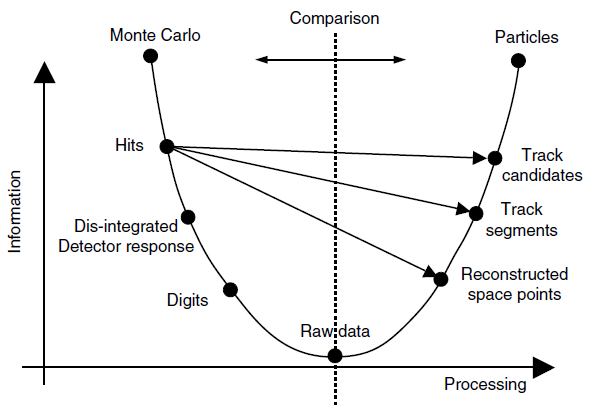
\includegraphics[width=10cm]{parabola.png}
\caption{Data processing framework taken from \cite{PPR1}}
\label{fig:parabola}
\end{figure}
Event generators create primary particles, depending on the physics one is interested in. Then, the physics processes at partonic level and informations such as type, momentum, charge, mother/daughter relationships... are stored in the kinematics tree. Different programmes are then used to simulate the transport of the particles through the detectors. During the transport, the energy deposition in the various detectors is stored as \textit{hits}. The hits are subsequently converted into \textit{digits}, which represent the real detector response and take into account instrumental effects, such as the noise due to the front-end electronics. Finally, the digit are stored in a specific hardware format for each detector as \textit{raw} data, that corresponds to the data format coming from the Data Acquisition System in a real data taking. \\From this point on the reconstruction starts, without distinguishing between real or simulate data. In the first step, the reconstructed points (rec points) are found for each detector by grouping the contiguous firing cells (clusterization) and then calculating the center of gravity of each cluster. The rec point is an estimation of the position where a particle crossed the sensitive area of the detector. The second step is the association of the rec points to tracks, which contain information on the kinematic variables, the identity and the energy loss of the particles. 

\subsubsection{Primary vertex reconstruction}
In ALICE, the primary vertex reconstruction is obtained using the two innermost silicon pixel layers of the ITS. The primary vertex position is the point where the two opposite bunches superimpose; while in the transverse plane, for the Pb-Pb collisions, the position of the beam is known with enough accuracy, along the z-axis, i.e. the beam line, a reconstruction of the vertex coordinate is needed on a event-by-event basis.  A first raw reconstruction of the primary vertex is done in order to give constraints in the successive tracking phase. The vertexing algorithm reconstructs hits in the two pixel layers that have a small difference in the azimuthal angle ($\phi <$ 0.01 rad) and in the pseudo-rapidity $\eta$, in order to select high momentum tracks only, with negligible multiple-scattering effects, and remove a huge combinatorial background. These linear tracks are called \textit{tracklets}. This algorithm was generalized to include reconstruction of all the three vertex coordinates. In fig. \ref{fig:vertexer} (left) the resolution of the reconstructed primary vertex using the SPD detector is shown as a function of number of tracklets for x,y and z coordinates in pp collisions. Typical values of resolution for heavy-ion collisions are 15 $\mu$m, while for pp collisions  they are of the order of 150 $\mu$m.
\begin{figure}[!t]
\begin{subfigure}{0.5\textwidth}
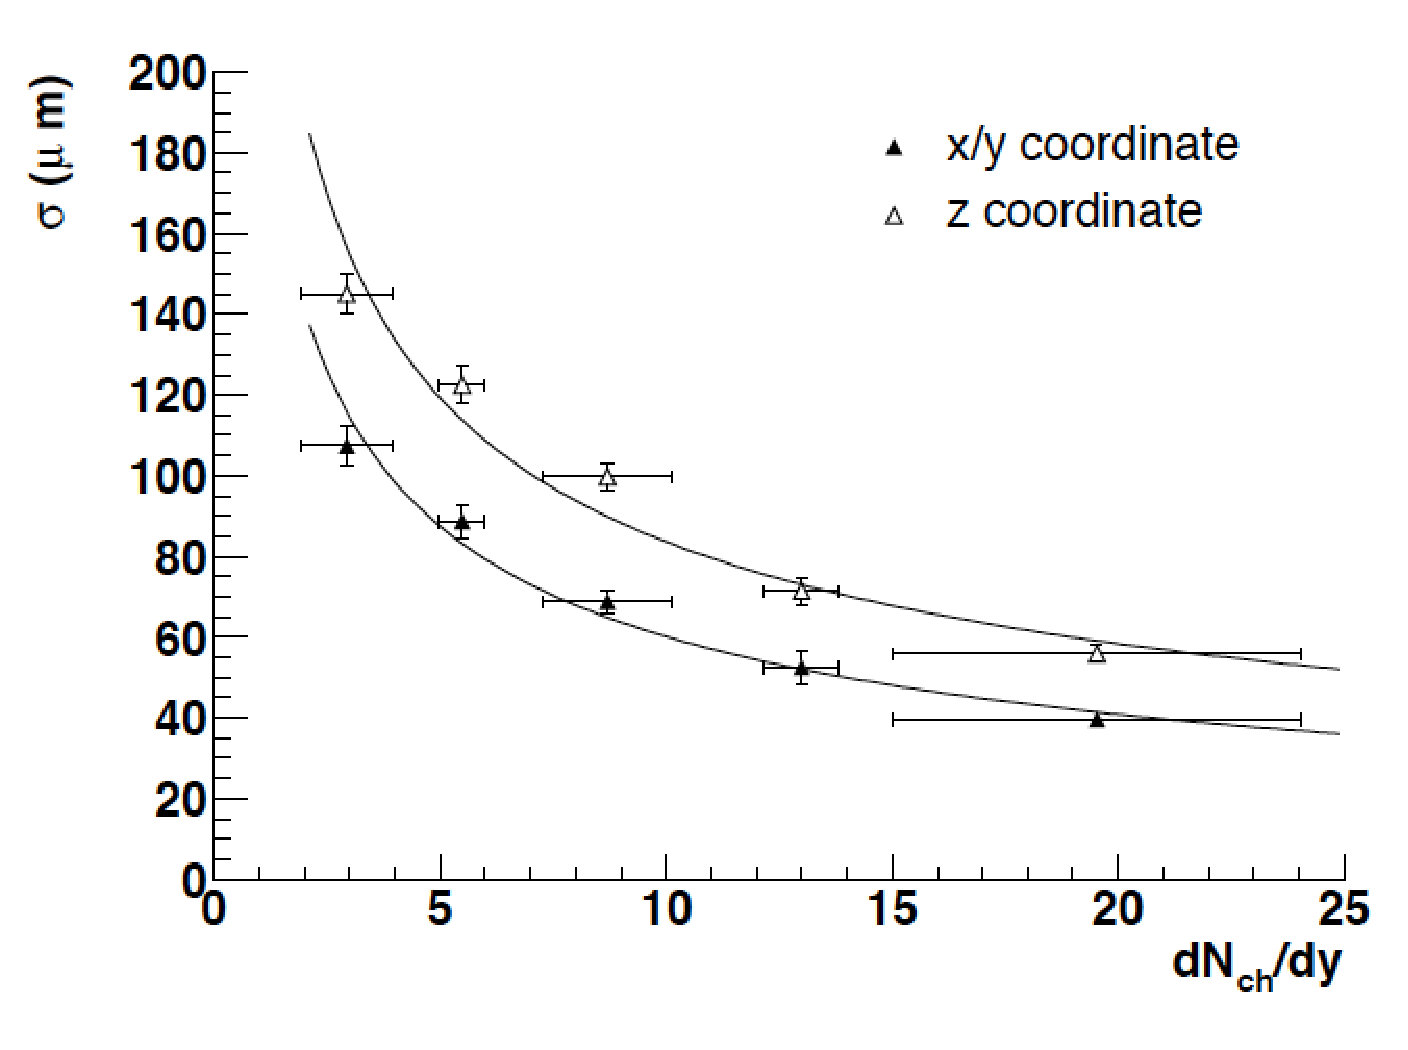
\includegraphics[width=7cm]{vertexPrim.pdf}
\end{subfigure}
\begin{subfigure}{0.5\textwidth}
\centering
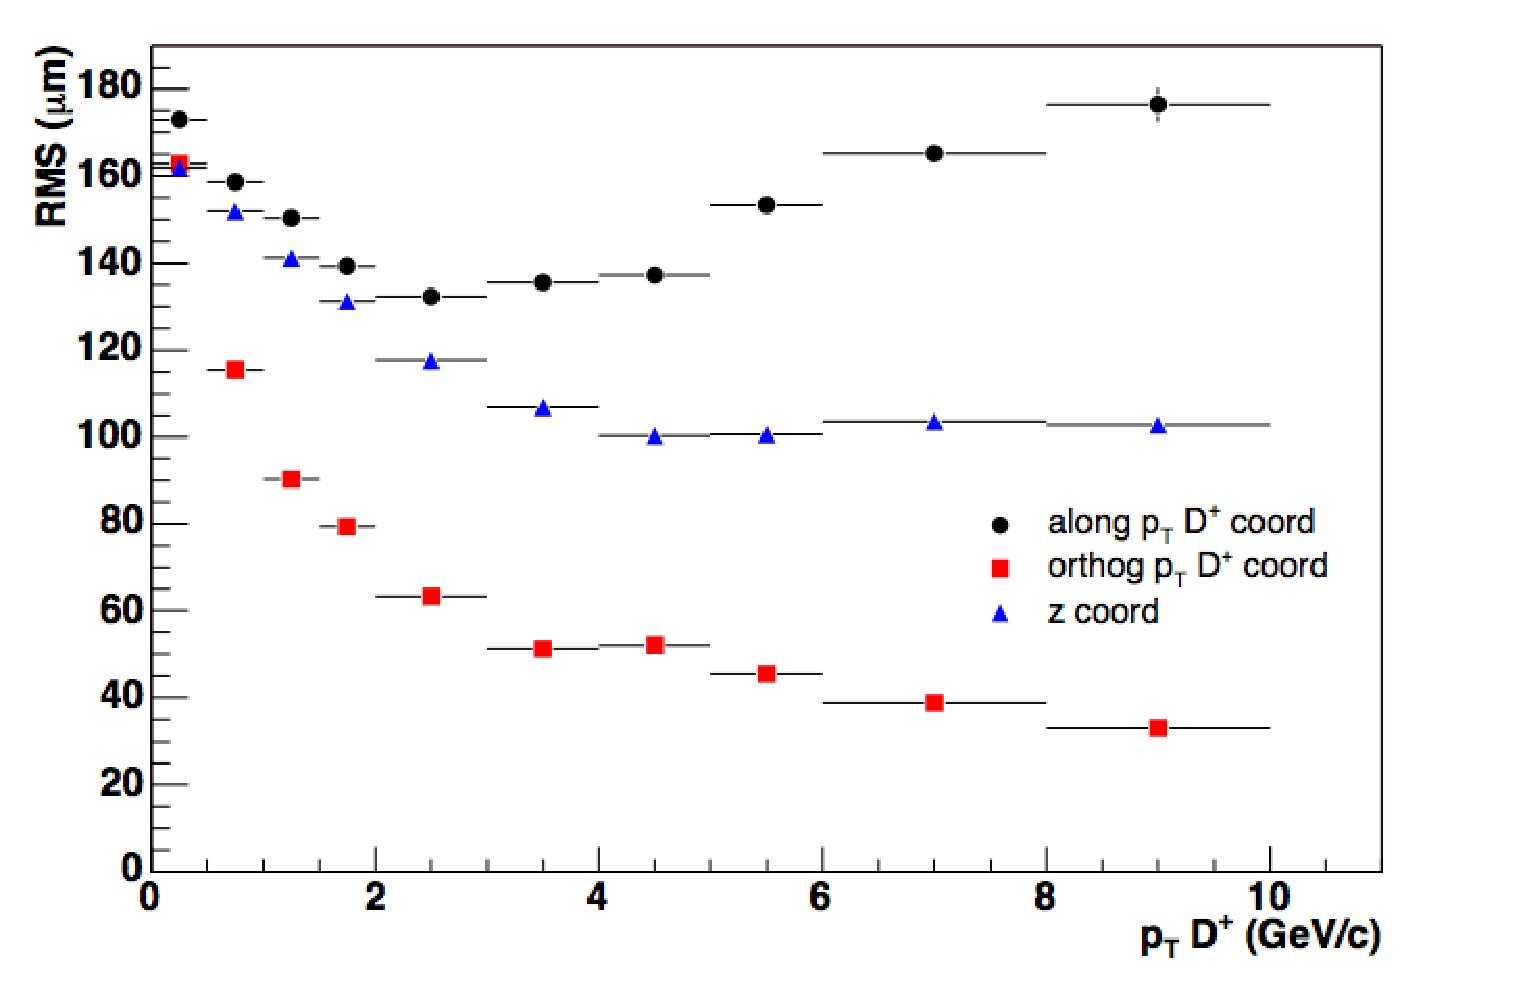
\includegraphics[width=7.5cm]{vertexSec.pdf}
\end{subfigure}
\caption{(Left) Resolution of the reconstructed primary vertex using the SPD detector as a function of number of tracklets for x, y and z coordinates in pp collisions. (Right) Resolution of the reconstructed secondary vertex along D$^+$ $p_t$ direction (black), orthogonal to D$^+$ $p_t$ direction (red), and along z-axis (blue). The resolution improves in the perpendicular plane to the D$^+$ $p_t$ direction.}
\label{fig:vertexer}
\end{figure}
After track reconstruction, the position of the primary vertex is recalculated using the measured track parameters. This second step is important in case of pp collisions because low multiplicity doesn't allow to have a sufficient precision in a first step, and also in case of analysis of charm and beauty decays, when one has to do with decay vertices displaced by few hundreds $\mu$m from the primary vertex. 

\subsubsection{Track reconstruction}
Track \textit{seeds} are created using the information from the TPC pad rows and the position of the SPD vertex. The track is propagated towards the inner radius of the TPC. Track candidates are then matched to the rec points in the outermost ITS layers and propagated down to the SPD, towards the primary vertex, estimated from SPD reconstructed points as
explained before, associating if possible new rec-points to the track. Once the primary vertex has been reached, the Kalman filter method is applied \cite{kalman}, again towards the outer detectors. In this way the track is propagated towards the TRD, TOF, HMPID, PHOS and EMCal detectors. Tracks with large $\chi^2$ are rejected. Finally the track is propagated backwards to the point of the closest approach to the primary vertex and track parameters are defined at this point.

\subsubsection{Secondary vertex reconstruction}
Tracks are grouped in triplets (for the $D^+_s$) following the charge ordering of the decay channel, defining objects called ``candidates''. The algorithm used is based on a straight line approximation of the tracks (which are helices): tracks are approximated as straight lines close to the primary vertex. The distance $d$ between the real secondary vertex and this line is sensitive to the discrepance between the helix and the straight line approximation; $d$ decreases with enlarging the transverse momenta and the distance between primary and secondary vertices. For each candidate a secondary vertex is computed as the point of closest approach between the reconstructed tracks. The algorithm finds the point of minimum distance between the three tracks by minimizing the quantity:
\begin{equation}
D^2=d^2_1+d^2_2+d^2_3
\end{equation}
where $d_i$ ($i$=1,2,3) is the distance between the track $i$ and the vertex ($x_0$, $y_0$, $z_0$), weighted with the errors on the track:
\begin{equation}
d^2_i=\left(\frac{x_i-x_0}{\sigma_{x_i}}\right)^2+
\left(\frac{y_i-y_0}{\sigma_{y_i}}\right)^2+\left(\frac{z_i-z_0}{\sigma_{z_i}}\right)^2\end{equation}
The resolution of the reconstructed secondary vertex is shown in fig. \ref{fig:vertexer} (right) as example for  the D$^+$ meson.
\fi